\begin{problem}
    \p
جمله عمومی دنباله زیر را به دست آورید.
	\p
    \begin{center}
     	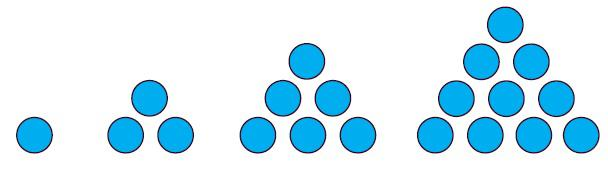
\includegraphics[scale=0.2]{./1.jpg}
    \end{center}
    \problemsolution{
        \p
       هر مثلث نسبت به مثلث قبلی یک ردیف بیشتر دارد یعنی:
       \begin{center}
       		\p 
    		$a_1 = 1$
    		\p
    		$a_2 = a_1 + 2$
    		\p
    		$a_3 = a_2 + 3$
    		\p
    		$     .       $
    		\p
    		$     .       $
    		\p
    		$     .       $
    		\p
    		$a_n = a_{n-1} + n$
    		\p
            $a_1 + a_2 + ... + a_n = a_1 + a_2 + ... + a_{n-1} + 1 + 2 + ... + n$
            \p
            $a_n = 1 + 2 + 3 + ... + n = \frac{n(n+1)}{2}$
        \end{center}
        }
\end{problem}